\begin{frame}
    \frametitle{Cámara de luz estructurada}

    \begin{figure}[!h]
        \centering
        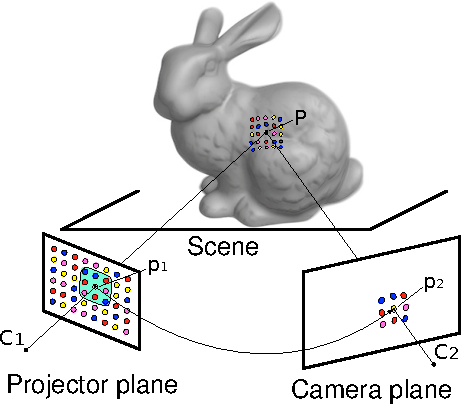
\includegraphics[width=0.4\columnwidth]{images/structured_light.pdf}
    \end{figure}

    La luz estructurada (\emph{structured light}) es el proceso de proyectar un patrón conocido de píxeles (ocasionalmente rejillas o barras horizontales) en una escena. La manera en que dicho patrón se deforma cuando golpea distintas superficies permite a los sistemas de visión calcular la profundidad e información de la superficie de los objetos en la escena.
\end{frame}